\chapter{Why}

\section{Doubt and Faith}

\keywords{compulsive thoughts, orientation of views, unexpected changes}

\noindent Sometimes we are interested in meditation in order to deal
with a disturbing or painful experience. We know something is wrong and
we can't shake it off. Or it could be a sense of feeling lost, where
nothing makes sense: such feelings keep returning, they don't let
themselves be ignored. Instead of answers, only the questions keep going
round and round: `Why does it have to be like this? What should I do,
and why? What's the point?'

Even in such confusion, merely acknowledging the state of our inner
chaos to ourselves already starts to provide some order and orientation.

\enlargethispage*{\baselineskip}

It is like driving on a road cluttered with trash. Slowing down to look
around is already much better than being blind to the dangerous clutter.
Our head is full of thoughts but only a few of them indicate reliable
directions, so we better examine them. Previously, we held a view that
things in our world were one way, but they have changed in a way we
didn't expect. It is not their fault, it is not our fault, but the
unexpected change is confusing, and we have to adjust our view.

Impermanence pulls the carpet out from under our feet, but at the same
time transforms our values, the qualities which we seek out as valuable
in our experiences. If we don't understand the change, it causes
confusion, followed by doubt. Even though we might know what we
\emph{should be doing}, we get stuck in the sense of doubt and
meaninglessness and we can't even begin.

\keywords{meaning, investigating what I believe, faith as fuel}

Why do you get up in the morning to do anything? Why does it matter at
all? If I keep asking `why' and dig into the layers of my constructed
self like this, the first layer reveals a matter of habit, `because this
is what I did yesterday'. Under that, the answers are formed out of
stories I tell myself about myself and the world I live in. Under that,
there is some degree of reasoning, philosophy and abstract ideas. Under
that, I am desperately trying to hold onto something solid, and I start
defending my ideas with personal memories and experiences (`because when
I was like this and this \ldots{}'), or I refer to famous names
(`because this and that teacher said \ldots{}').

Under that, I have to give up and confess that it is a matter of faith
and personal conviction. What I do is simply what I decide there and
then. At the end, I stand there and have to admit that I don't
\emph{know}, but I \emph{believe} that doing such-and-such makes sense.

Faith is not a fixed quality in the mind. We have the capacity to choose
credible statements which we perceive will guide us toward a greater
understanding and happiness. We can test any given belief by applying it
in practice and by observing the results, and we can then support or
abandon that belief accordingly.

I may review, investigate and update \emph{what I believe} about what
makes sense to me, but until my experience verifies it, my reasoning has
to be supported by faith. Otherwise, I will not make an effort in any
direction, and my life will be governed by blind habits and external
pressures.

Faith is the fuel for the virtues of resolve and energy. Later on, faith
will be reinforced by experiencing the results of practice, but without
fuel, our car doesn't even start.

\keywords{belief as a cause of action, trust in the teacher}

A belief creates a cause for an action. Without that belief, I don't
take that action. In the Buddhist perspective, there are two fundamental
beliefs:

\begin{enumerate}
\item
  A phenomena occurs when the sufficient causes for it are present; and
  it either does not occur, or it ceases, when the sufficient causes are
  absent.\footnote{\href{https://www.dhammatalks.org/suttas/SN/SN12_61.html}{SN
    12.61}, Uninstructed}
\item
  The Buddha completely understood the truth about the way things are,
  and thus freed himself from greed, hatred and delusion. Hence he is an
  excellent teacher of the way of practice.
\end{enumerate}

The Buddha gave us the instruction that each person should question,
ponder, and investigate the way things really are to understand it for
themselves. Nonetheless, how are we going to start? Without trust in the
teacher, we are lost in the tangle of our personal opinions and it is
unlikely that we are going to listen and learn anything new. The
tradition reminds us of this relation to faith when, before giving a
Dhamma talk, we start by chanting \emph{namo tassa} three times.

\begin{quote}
\emph{Namo tassa bhagavato arahato sammā-sambuddhassa}

Homage to the Blessed, Noble, and Perfectly Enlightened One.
\end{quote}

\keywords{doubt, wandering in a desert, grasping creates limits}

The Buddha compared doubt to being lost in a desert, wandering around
without water.\footnote{\href{https://suttacentral.net/dn2}{DN 2}, The
  Fruits of the Ascetic Life} Everything else is secondary: we can only
think about how to find water and escape the desert.

Or, we fantasize about how to comfortably numb the mind and not think
about anything at all, `tranquillizing oneself with the
trivial'\footnote{Søren Kierkegaard, `The Sickness Unto Death'} to
continue everything as normal. In doubt, it is not clear how we will
escape this situation, but we can start by acknowledging the aspiration
to be well and to live a happy life.

It is our natural human ability to overcome confusion and develop
long-term happiness in our lives. A long-term view has to include
changes to our situation, loss and tragedy. Stable happiness has to be
founded on a perspective which integrates impermanence.

In the \emph{suttas}, doubt appears both in the list of Five Hindrances,
and in the first three of the Ten Fetters, which are the ones that
obscure understanding the Four Noble Truths. When doubt gets personal,
there is no doubt that it leads to suffering. Figures
\ref{fig-leading-to-suffering} and \ref{fig-leading-to-cessation}
illustrate how we get into this mess, and how we can get out of it.

As a hindrance, doubt stops Right Effort, and stops developing the mind.
As a fetter, it compels us to keep looking for fixed certainties, and
thus ties us even tighter to our ideas about who we are.

We like the suggestion to develop our mind, but initially, we think this
means making sure who and what we are, getting more of what we need, or
changing ourselves to become something different.

`Who am I? What am I? What should I do? Is this the right thing? Or is
it something else?' This way of thinking is a trap, it goes round and
round with no way out. All these concerns are tied up with holding onto
some kind of identity which will again invite doubt. Until we realize
what is happening, we are caught in the cycle.

Even when we become successful, at the end of that becoming, it is going
to change according to its nature, and we find that our new identity is
also hollow, empty of real value, just as our previous idea of ourself.

Grasping at and holding onto what we think we are, being afraid to let
go: this is the obstruction. This creates the very limit we are
frustratedly running up against. Understanding freedom through letting
go doesn't come to us easily.

\cleartoverso
\figurepagelayout

\begin{figure}[h]
\vspace*{-10mm}%
\caption{Leading to Suffering}\label{fig-leading-to-suffering}

\centering

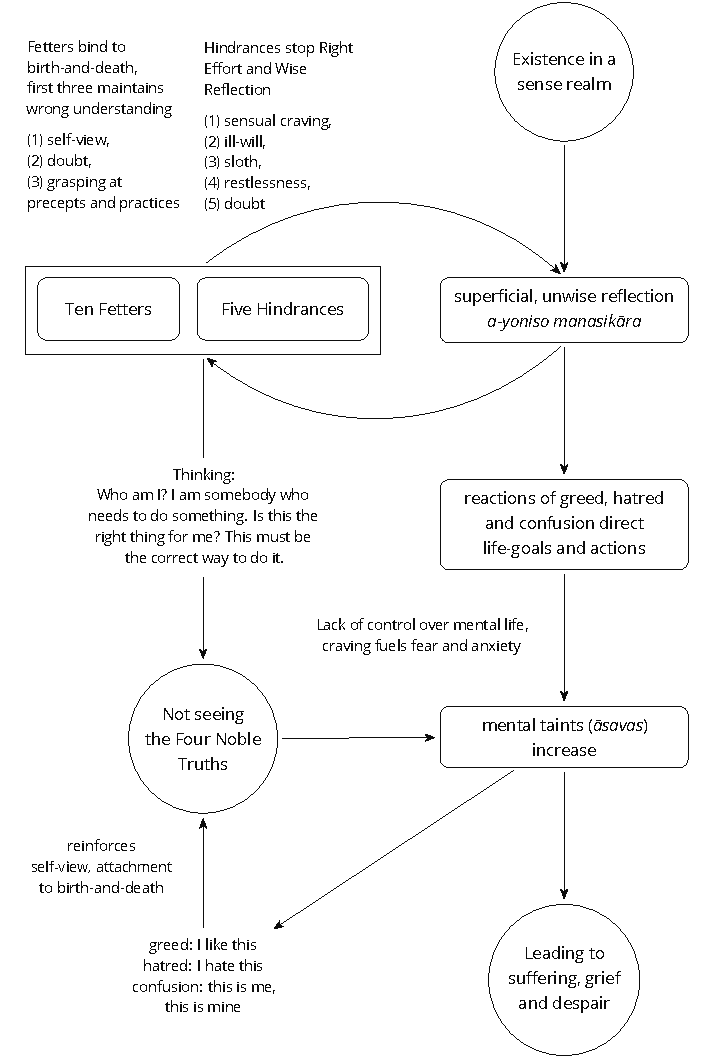
\includegraphics[width=\linewidth]{./manuscript/tex/diagrams/leading-to-suffering.pdf}

\end{figure}

\clearpage

\begin{figure}[h]
\vspace*{-10mm}%
\caption{Leading to Cessation}\label{fig-leading-to-cessation}

\centering

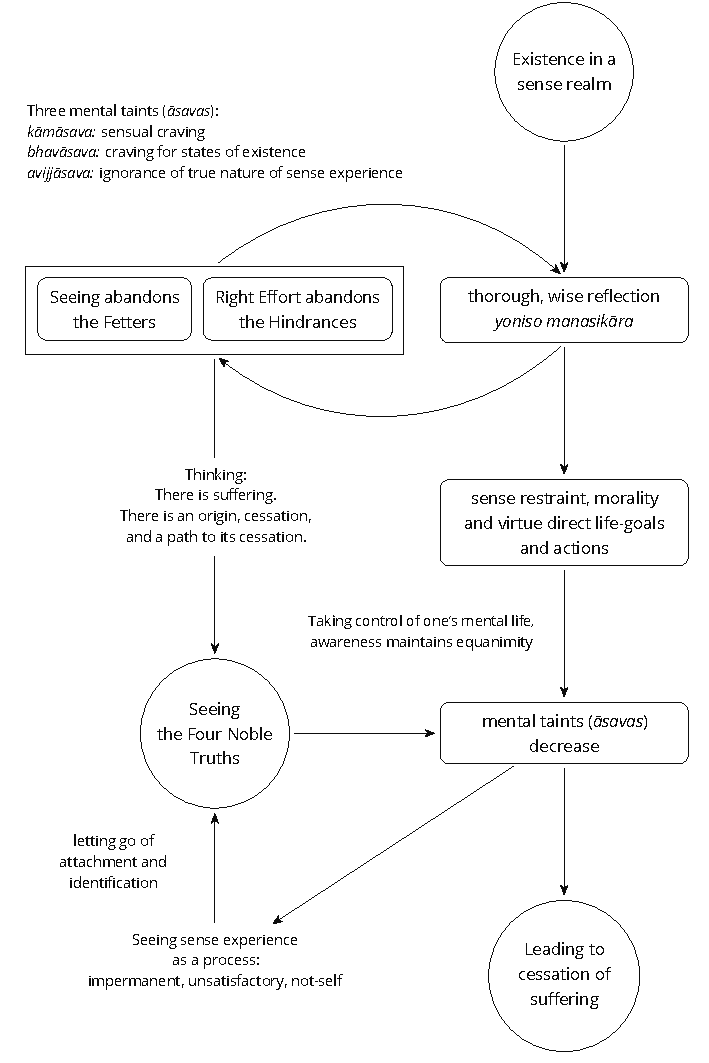
\includegraphics[width=\linewidth]{./manuscript/tex/diagrams/leading-to-cessation.pdf}

\end{figure}

\clearpage
\normalpagelayout

\section{Right View}

\keywords{returning to the beginning, observing thoughts}

\noindent Let's return to the breath and continue the meditation
practice. At the beginning of a session, start with the basics, simple
steps which guide the attention back to the familiar frame: the in- and
out breath, the body and its feelings. Observe what you are experiencing
as a process which is going through continuos change from one feeling
into another.

Every meditation session is a new beginning, we can't save the results
of the previous session and load in the knowledge. If we start thinking
we already know, say, if we have been practising this for years, this
results in a closed attitude which blocks even our earlier
understanding. Our experience from the past is only relevant when we
apply it to the present. The changing present keeps understanding fresh
and new.

`This thought, this feeling had a beginning, it is changing now, it will
cease and end. Can I wait and notice that cessation?' Contemplating
direct experience this way, the mind gives up its desire and fear
regarding particular states, and understands them as part of natural
processes. We are not reasoning to ourselves about what we think about
the mind, rather, as if taking a step back and watching it, we mindfully
experience the way it is.

\enlargethispage*{2\baselineskip}

This contemplation restores Right View, as if someone took an upside
down flower vase standing on its top, and put it upright again. When we
look, we understand which part of the vase is the top and which the
bottom. We crave and want to hold onto experiences that are always going
to change, doesn't that sound stressful? Fortunately the mistake is
avoidable.

\clearpage

\keywords{freedom around limitations, essentials, gratitude, flooded with good advice}

Right View finds space and freedom around the limitations and pressures
of life. At first, we might not see much open space, but contemplating
the essentials, we might notice that we don't need everything we can
think of. We can ask, `Do I have what I need for this single day?'

We can take stock of what we are using in our immediate environment --
clothing, food, shelter, medicine. Sometimes, others give them to us or
allow us to use them. At other times, we give them to others. `Do I know
how much is enough for today?' A sense of calmness returns when I
recollect them again, even though I might know these fact already.

Recollecting the simple things, that we have what we need to live this
day well, our attitude expresses itself in feelings of contentment and
gratitude for life. You don't have to ask for them and you can't create
them by will. We have to make space for them in our view, then they
arise on their own.

What's the great hurry for? A simple exercise is to stop and do nothing
for two minutes, not looking for entertainment and distraction. You can
watch the breath, but this is optional. Not rejecting boredom as a
mental state increases our focus and preserves energy.

The problem is not that we don't know enough. The bookshelves are
overflowing with good advice about `how to be happy'. If that's all we
need, where is the problem? If all it took was good advice, all of us
would have gotten enlightened long ago. We hear and read about all the
good things we should do and what sort of person we should be: one book
says we should be tough and fearless, while another says we should have
universal compassion. It is a special kind of suffering to read it all.

Or perhaps we need \emph{Nibbāna}? Is that the right idea? The meaning
of the word is `going cool', as in a fire ceasing to burn and growing
cool. A craving to `have it' means more fuel for the heat and burning of
becoming.

But \emph{Nibbāna} is the coolness of ceasing to burn with becoming, so
should we become this non-becoming? The thinking mind goes,
`\emph{What?!}' And that's not a wrong answer either: the teaching of
the Buddha points out that thinking and becoming are not sufficient
tools here. Any other state or thought, when we see ourselves in it,
will be as limiting as the previous one. We are not freed by
\emph{becoming} the right thing, but by recognizing that we can give up
the compulsion to continue becoming.

\clearpage
\figurepagelayout

\begin{figure}[h]
\caption{Experience, Becoming and the Deathless}\label{fig-experience-becoming-deathless}
\bigskip
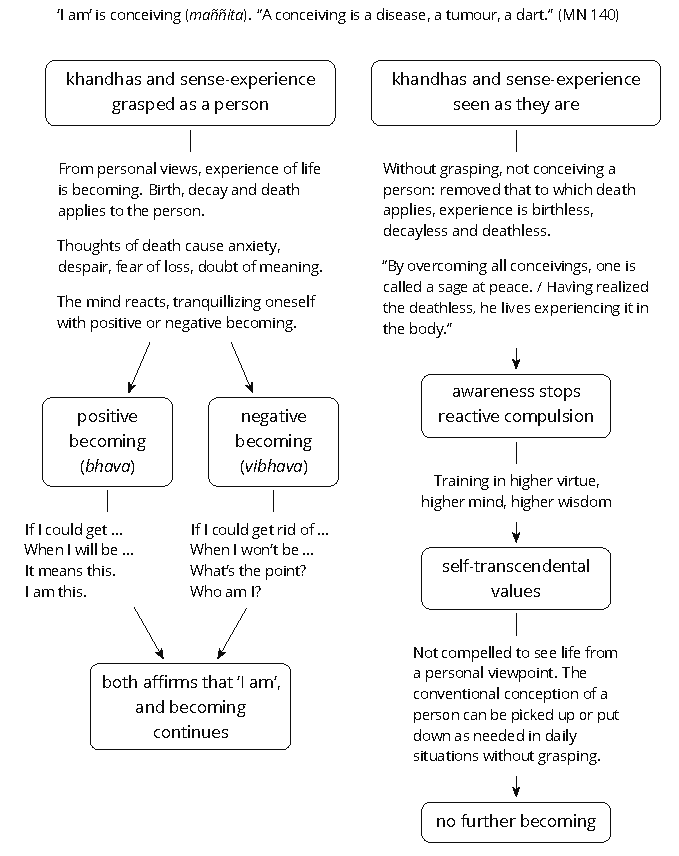
\includegraphics[width=\linewidth]{./manuscript/tex/diagrams/experience-becoming-deathless.pdf}
\end{figure}

{\noindent\footnotesize
See also: Chapter 10, Birth, Decay and Death in The Buddha's Teaching: It's Essential\\ Meaning by R. G. de S. Wettimuny
\par}

% TODO: link to Wettimuny book

\clearpage
\normalpagelayout

\section{New Eyes}

\keywords{turning toward experience, intellectual knowledge, watching the senses}

\noindent We can turn a compulsive tendency into meditation practice by
asking, `How can I understand this experience?' This question directs us
to the noble attitude towards suffering described in the Four Noble
Truths: `Suffering should be understood.' Discard the opinions which
present themselves as answers, and keep returning to this open attitude
of knowing the present.

Both joy and sorrow are natural processes, but if we don't understand
them, we see one as a reward and the other as a punishment. Life never
seems to be fair and it always seems to be out of our control.

To open up our attitude for contemplation, we can at least imagine the
possibility that there is something here we can learn. A turning point
occurs when we are able to let go of being sure about our opinions and
can stop to investigate the experience itself.

Consider how narrow our attitude is when we start with the thought,
`I've seen this, I know this'. Perhaps this is true, but I notice that
when I try to use that intellectual knowledge to solve a problem, my
attention merely revolves around memories, thoughts and opinions. While
I am caught up in the past, the present experience escapes my attention.

The instruction of the Buddha is to establish a careful intention to
meditate, and to put aside the matters of the world.

\clearpage

\begin{quote}
There is the case where a monk remains focused \ldots{} ardent, alert,
and mindful -- subduing greed and distress with reference to the world.

\bigskip

\quoteRef{%

\href{https://suttacentral.net/mn10}{MN 10}, Mindfulness Meditation

}
\end{quote}

The thoughts and opinions don't become `our knowledge', but we can
understand the process of their arising and ceasing. `\emph{What} is it
that I am doing? \emph{How} am I doing it?' Letting go of our fixed
positions becomes the way forward; we discover it by seeing with new
eyes.\footnote{`The real voyage of discovery consists not in seeking new
  landscapes, but in having new eyes.' (Marcel Proust)} Life may still
not be fair or entirely under our control, but now we are familiar with
a practice which makes the difference between knowing mental states and
having a mental breakdown.

The fundamental principle is that watching the mind develops the mind. A
wakeful awareness unbinds the compulsive tendencies. We cannot know what
is going to happen tomorrow, but there will be change. The word `Buddha'
means `one who knows, one who is awake'. The source of contentment in
activity is that we continue to trust and practice living in this
wakeful awareness.
